\documentclass{standalone}
\usepackage{tikz}
\usetikzlibrary{patterns, positioning}


\begin{document}
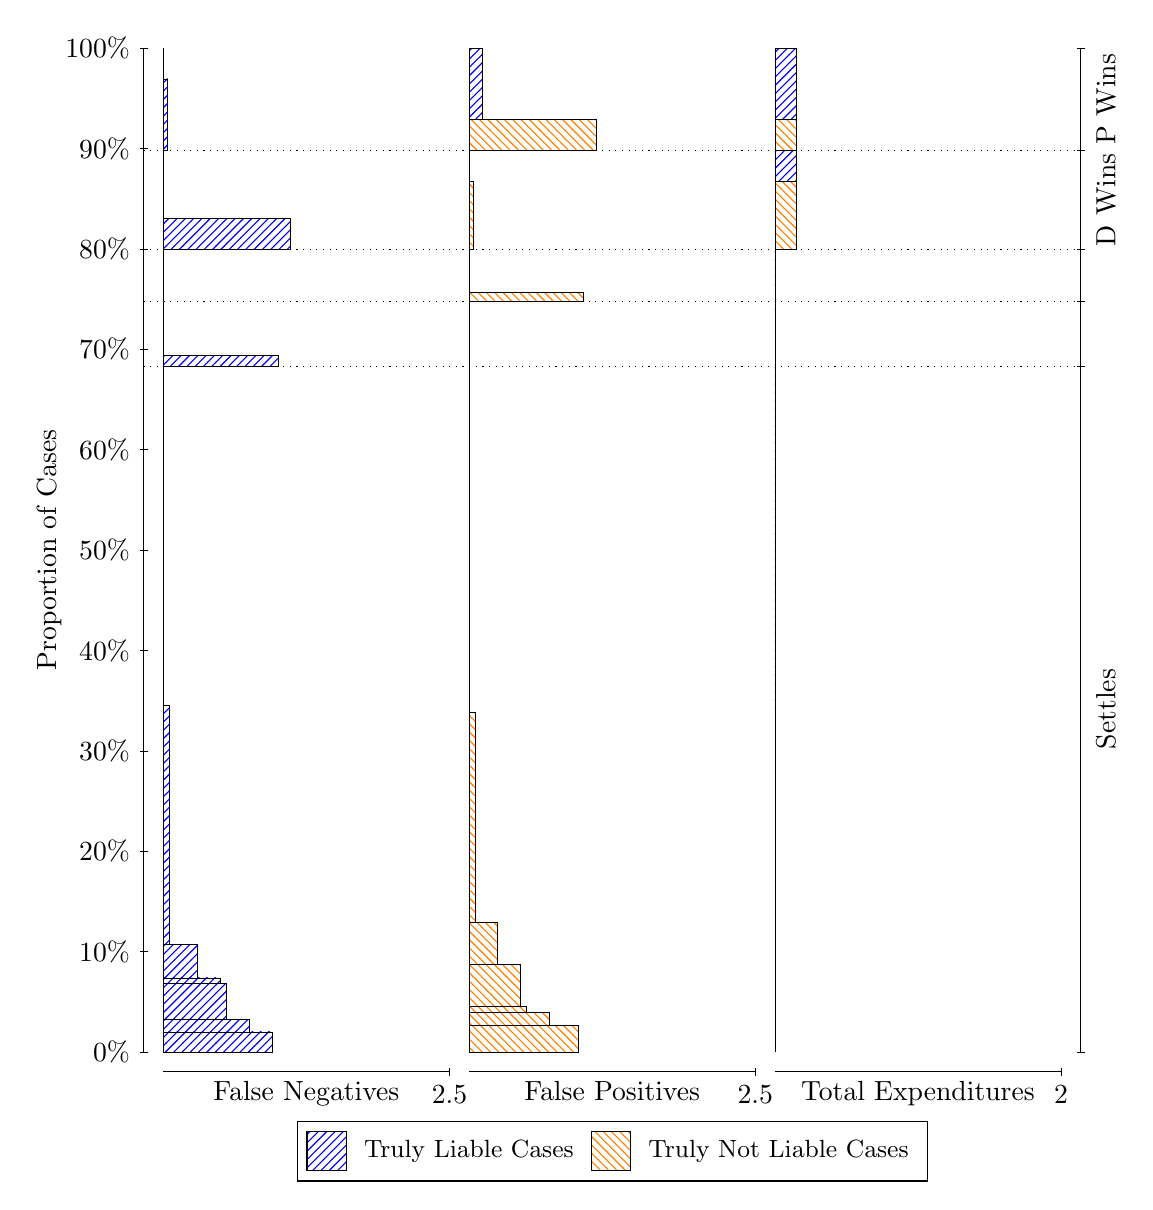
\begin{tikzpicture}
\draw[black, very thin] (1.5,1.75) -- (1.5,14.5);
\node[rotate=90, text=black, anchor=center] at (0.3, 8.125) {Proportion of Cases};
\draw[black, very thin] (1.45,1.75) -- (1.55,1.75);
\node[text=black, anchor=east] at (1.45, 1.75) {0\%};
\draw[black, very thin] (1.45,3.025) -- (1.55,3.025);
\node[text=black, anchor=east] at (1.45, 3.025) {10\%};
\draw[black, very thin] (1.45,4.3) -- (1.55,4.3);
\node[text=black, anchor=east] at (1.45, 4.3) {20\%};
\draw[black, very thin] (1.45,5.575) -- (1.55,5.575);
\node[text=black, anchor=east] at (1.45, 5.575) {30\%};
\draw[black, very thin] (1.45,6.85) -- (1.55,6.85);
\node[text=black, anchor=east] at (1.45, 6.85) {40\%};
\draw[black, very thin] (1.45,8.125) -- (1.55,8.125);
\node[text=black, anchor=east] at (1.45, 8.125) {50\%};
\draw[black, very thin] (1.45,9.4) -- (1.55,9.4);
\node[text=black, anchor=east] at (1.45, 9.4) {60\%};
\draw[black, very thin] (1.45,10.675) -- (1.55,10.675);
\node[text=black, anchor=east] at (1.45, 10.675) {70\%};
\draw[black, very thin] (1.45,11.95) -- (1.55,11.95);
\node[text=black, anchor=east] at (1.45, 11.95) {80\%};
\draw[black, very thin] (1.45,13.225) -- (1.55,13.225);
\node[text=black, anchor=east] at (1.45, 13.225) {90\%};
\draw[black, very thin] (1.45,14.5) -- (1.55,14.5);
\node[text=black, anchor=east] at (1.45, 14.5) {100\%};

\draw[black, very thin] (13.4,1.75) -- (13.4,14.5);
\draw[black, very thin] (13.35,1.75) -- (13.45,1.75);
\node[anchor=west] at (13.35, 1.75) {};
\draw[black, very thin] (13.35,10.46) -- (13.45,10.46);
\node[anchor=west] at (13.35, 10.46) {};
\draw[black, very thin] (13.35,11.284) -- (13.45,11.284);
\node[anchor=west] at (13.35, 11.284) {};
\draw[black, very thin] (13.35,11.94) -- (13.45,11.94);
\node[anchor=west] at (13.35, 11.94) {};
\draw[black, very thin] (13.35,13.201) -- (13.45,13.201);
\node[anchor=west] at (13.35, 13.201) {};
\draw[black, very thin] (13.35,14.5) -- (13.45,14.5);
\node[anchor=west] at (13.35, 14.5) {};

\draw[black, very thin, pattern color=blue, pattern=north east lines] (1.75,1.75) rectangle (3.1307,2.0065);
\draw[black, very thin, pattern color=blue, pattern=north east lines] (1.75,2.0065) rectangle (2.84,2.1661);
\draw[black, very thin, pattern color=blue, pattern=north east lines] (1.75,2.1661) rectangle (2.5493,2.6212);
\draw[black, very thin, pattern color=blue, pattern=north east lines] (1.75,2.6212) rectangle (2.4767,2.6896);
\draw[black, very thin, pattern color=blue, pattern=north east lines] (1.75,2.6896) rectangle (2.186,3.1148);
\draw[black, very thin, pattern color=blue, pattern=north east lines] (1.75,3.1148) rectangle (1.8227,6.152);
\draw[black, very thin, pattern color=orange, pattern=north west lines] (1.75,6.152) rectangle (1.75,10.46);
\draw[black, very thin, pattern color=blue, pattern=north east lines] (1.75,10.46) rectangle (3.2033,10.595);
\draw[black, very thin, pattern color=orange, pattern=north west lines] (1.75,10.595) rectangle (1.75,11.284);
\draw[black, very thin, pattern color=orange, pattern=north west lines] (1.75,11.284) rectangle (1.75,11.4);
\draw[black, very thin, pattern color=blue, pattern=north east lines] (1.75,11.4) rectangle (1.75,11.94);
\draw[black, very thin, pattern color=blue, pattern=north east lines] (1.75,11.94) rectangle (3.3668,12.332);
\draw[black, very thin, pattern color=orange, pattern=north west lines] (1.75,12.332) rectangle (1.75,13.201);
\draw[black, very thin, pattern color=blue, pattern=north east lines] (1.75,13.201) rectangle (1.8045,14.108);
\draw[black, very thin, pattern color=orange, pattern=north west lines] (1.75,14.108) rectangle (1.75,14.5);
\draw[black, very thin, pattern color=orange, pattern=north west lines] (5.6333,1.75) rectangle (7.014,2.0889);
\draw[black, very thin, pattern color=orange, pattern=north west lines] (5.6333,2.0889) rectangle (6.6507,2.2534);
\draw[black, very thin, pattern color=orange, pattern=north west lines] (5.6333,2.2534) rectangle (6.36,2.3327);
\draw[black, very thin, pattern color=orange, pattern=north west lines] (5.6333,2.3327) rectangle (6.2873,2.8599);
\draw[black, very thin, pattern color=orange, pattern=north west lines] (5.6333,2.8599) rectangle (5.9967,3.3939);
\draw[black, very thin, pattern color=orange, pattern=north west lines] (5.6333,3.3939) rectangle (5.706,6.058);
\draw[black, very thin, pattern color=blue, pattern=north east lines] (5.6333,6.058) rectangle (5.6333,10.46);
\draw[black, very thin, pattern color=orange, pattern=north west lines] (5.6333,10.46) rectangle (5.6333,11.149);
\draw[black, very thin, pattern color=blue, pattern=north east lines] (5.6333,11.149) rectangle (5.6333,11.284);
\draw[black, very thin, pattern color=orange, pattern=north west lines] (5.6333,11.284) rectangle (7.0867,11.4);
\draw[black, very thin, pattern color=blue, pattern=north east lines] (5.6333,11.4) rectangle (5.6333,11.94);
\draw[black, very thin, pattern color=orange, pattern=north west lines] (5.6333,11.94) rectangle (5.6878,12.809);
\draw[black, very thin, pattern color=blue, pattern=north east lines] (5.6333,12.809) rectangle (5.6333,13.201);
\draw[black, very thin, pattern color=orange, pattern=north west lines] (5.6333,13.201) rectangle (7.2502,13.594);
\draw[black, very thin, pattern color=blue, pattern=north east lines] (5.6333,13.594) rectangle (5.7968,14.5);
\draw[black, very thin, pattern color=orange, pattern=north west lines] (9.5167,1.75) rectangle (9.5167,6.058);
\draw[black, very thin, pattern color=blue, pattern=north east lines] (9.5167,6.058) rectangle (9.5167,10.46);
\draw[black, very thin, pattern color=orange, pattern=north west lines] (9.5167,10.46) rectangle (9.5167,11.149);
\draw[black, very thin, pattern color=blue, pattern=north east lines] (9.5167,11.149) rectangle (9.5167,11.284);
\draw[black, very thin, pattern color=orange, pattern=north west lines] (9.5167,11.284) rectangle (9.5167,11.4);
\draw[black, very thin, pattern color=blue, pattern=north east lines] (9.5167,11.4) rectangle (9.5167,11.94);
\draw[black, very thin, pattern color=orange, pattern=north west lines] (9.5167,11.94) rectangle (9.7892,12.809);
\draw[black, very thin, pattern color=blue, pattern=north east lines] (9.5167,12.809) rectangle (9.7892,13.201);
\draw[black, very thin, pattern color=orange, pattern=north west lines] (9.5167,13.201) rectangle (9.7892,13.594);
\draw[black, very thin, pattern color=blue, pattern=north east lines] (9.5167,13.594) rectangle (9.7892,14.5);
\draw[black, dotted] (1.5,10.46) -- (13.4,10.46);
\draw[black, dotted] (1.5,11.284) -- (13.4,11.284);
\draw[black, dotted] (1.5,11.94) -- (13.4,11.94);
\draw[black, dotted] (1.5,13.201) -- (13.4,13.201);
\draw[black, very thin] (1.75,1.5) -- (5.3833,1.5);
\node[text=black, anchor=north] at (3.5667, 1.5) {False Negatives};
\draw[black, very thin] (5.3833,1.45) -- (5.3833,1.55);
\node[text=black, anchor=north] at (5.3833, 1.45) {2.5};

\draw[black, very thin] (5.6333,1.5) -- (9.2667,1.5);
\node[text=black, anchor=north] at (7.45, 1.5) {False Positives};
\draw[black, very thin] (9.2667,1.45) -- (9.2667,1.55);
\node[text=black, anchor=north] at (9.2667, 1.45) {2.5};

\draw[black, very thin] (9.5167,1.5) -- (13.15,1.5);
\node[text=black, anchor=north] at (11.333, 1.5) {Total Expenditures};
\draw[black, very thin] (13.15,1.45) -- (13.15,1.55);
\node[text=black, anchor=north] at (13.15, 1.45) {2};

\node[text=black, centered, rotate=90] at (13.72, 6.105) {Settles};


\node[text=black, centered, rotate=90] at (13.72, 12.571) {D Wins};
\node[text=black, centered, rotate=90] at (13.72, 13.851) {P Wins};

\draw (7.449999999999999,1.5) node[draw=none] (baseCoordinate) {};
\begin{scope}[align=center]
        \matrix[scale=0.5, draw=black, below=0.5cm of baseCoordinate, nodes={draw}, column sep=0.1cm]{
            \node[rectangle, draw, minimum width=0.5cm, minimum height=0.5cm, pattern color=blue, pattern=north east lines] {}; &
            \node[draw=none, font=\small, text=black] (B) {Truly Liable Cases}; &
            \node[rectangle, draw, minimum width=0.5cm, minimum height=0.5cm, pattern color=orange, pattern=north west lines] {}; &
            \node[draw=none, font=\small, text=black] (B) {Truly Not Liable Cases}; \\
            };
\end{scope}

\end{tikzpicture}
\end{document}